\documentclass[11pt,a4paper]{article}
\usepackage[margin=1in]{geometry}
\usepackage{tikz}
\usepackage{booktabs}
\usepackage{longtable}
\usepackage{xcolor}
\usepackage{enumitem}

\usetikzlibrary{shapes.geometric, arrows.meta, positioning, fit, calc}

\tikzset{
  callback/.style={rectangle, draw=green!60!black, fill=green!5, thick, rounded corners, minimum width=2.2cm, align=center, font=\small\bfseries},
  nocallback/.style={rectangle, draw=gray, fill=gray!10, rounded corners, minimum width=2.2cm, align=center, font=\small},
  decision/.style={diamond, draw=blue!60, fill=blue!5, aspect=2, align=center, font=\small},
  arrow/.style={-{Stealth[length=2mm]}, thick},
  label/.style={font=\scriptsize, fill=white, inner sep=1pt}
}

\begin{document}

\begin{center}
{\LARGE \textbf{Compare Flow: Graph \& Callback Nodes}}\\[0.5em]
{\large (resume\_url in payload)}
\end{center}

\vspace{1em}
When \texttt{resume\_url} is present and the request is a compare flow (\texttt{/compare-candidate-job}, \texttt{request\_type=candidate\_job\_match}), the graph runs the following path. \textbf{Green} = sends callback; \textbf{Gray} = no callback.

\vspace{1.5em}

\begin{center}
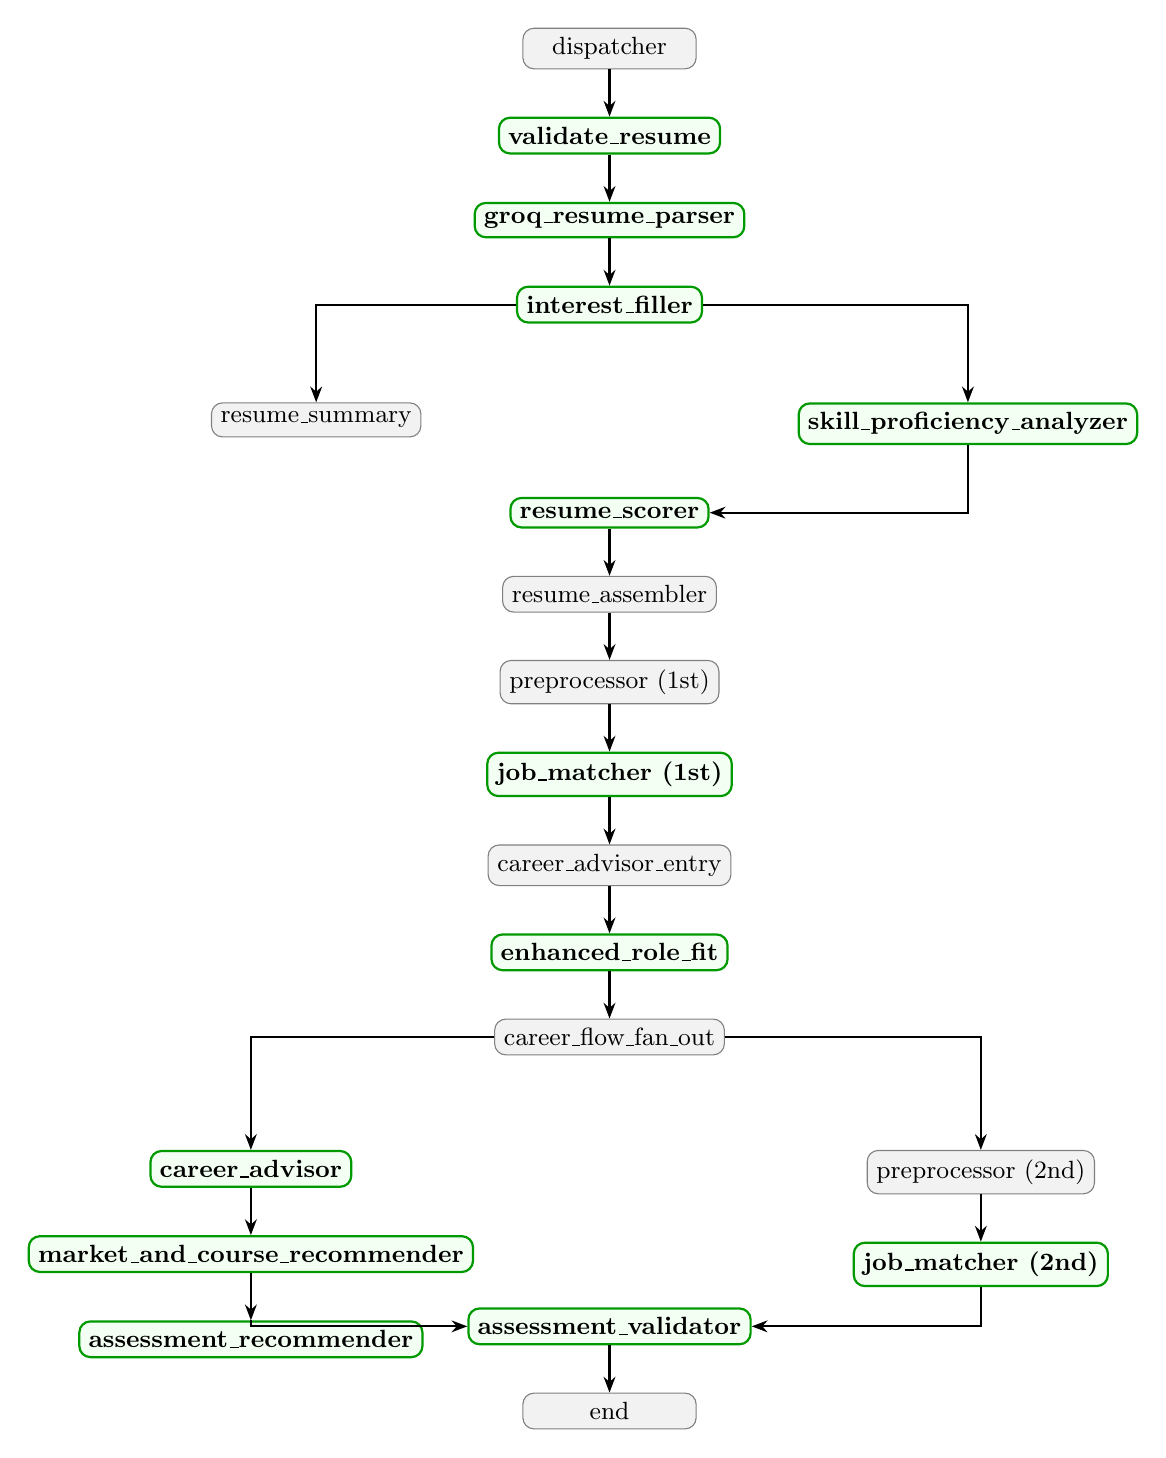
\begin{tikzpicture}[node distance=0.6cm and 1.2cm]

  % Entry
  \node[nocallback] (disp) {dispatcher};

  % Stage 1
  \node[callback, below=of disp] (val) {validate\_resume};
  \node[callback, below=of val] (groq) {groq\_resume\_parser};
  \node[callback, below=of groq] (int) {interest\_filler};

  % Parallel branch
  \node[nocallback, below left=1cm and 1.2cm of int] (sum) {resume\_summary};
  \node[callback, below right=1cm and 1.2cm of int] (skill) {skill\_proficiency\_analyzer};

  % Resume scorer (before assembler)
  \node[callback, below=2.2cm of int] (rs) {resume\_scorer};
  \node[nocallback, below=of rs] (asm) {resume\_assembler};

  % Job matcher 1st run
  \node[nocallback, below=of asm] (pre1) {preprocessor (1st)};
  \node[callback, below=of pre1] (jm1) {job\_matcher (1st)};

  % Unified flow: career_advisor_entry -> enhanced_role_fit (same as normal resume)
  \node[nocallback, below=of jm1] (cae) {career\_advisor\_entry};
  \node[callback, below=of cae] (erf) {enhanced\_role\_fit};

  % Fan out (parallel: career + job matcher)
  \node[nocallback, below=of erf] (fan) {career\_flow\_fan\_out};

  % Parallel branches
  \node[callback, below left=1.2cm and 1.8cm of fan] (ca) {career\_advisor};
  \node[nocallback, below right=1.2cm and 1.8cm of fan] (pre2) {preprocessor (2nd)};

  \node[callback, below=of ca] (mkt) {market\_and\_course\_recommender};
  \node[callback, below=of pre2] (jm2) {job\_matcher (2nd)};

  \node[callback, below=of mkt] (ar) {assessment\_recommender};

  % Both branches converge to assessment_validator (fan-in guard skips until both ready)
  \node[callback, below=3.2cm of fan] (av) {assessment\_validator};
  \node[nocallback, below=of av] (end) {end};

  % Arrows
  \draw[arrow] (disp) -- (val);
  \draw[arrow] (val) -- (groq);
  \draw[arrow] (groq) -- (int);
  \draw[arrow] (int) -| (sum);
  \draw[arrow] (int) -| (skill);
  \draw[arrow] (skill) |- (rs);
  \draw[arrow] (rs) -- (asm);
  \draw[arrow] (asm) -- (pre1);
  \draw[arrow] (pre1) -- (jm1);
  \draw[arrow] (jm1) -- (cae);
  \draw[arrow] (cae) -- (erf);
  \draw[arrow] (erf) -- (fan);
  \draw[arrow] (fan) -| (ca);
  \draw[arrow] (fan) -| (pre2);
  \draw[arrow] (ca) -- (mkt);
  \draw[arrow] (pre2) -- (jm2);
  \draw[arrow] (mkt) -- (ar);
  \draw[arrow] (ar) |- (av);
  \draw[arrow] (jm2) |- (av);
  \draw[arrow] (av) -- (end);

\end{tikzpicture}
\end{center}

\vspace{2em}

\section*{Nodes That Send Callbacks (12 total)}

\begin{enumerate}[nosep]
  \item \texttt{validate\_resume} -- resume validation result
  \item \texttt{groq\_resume\_parser} -- parsed structured resume
  \item \texttt{interest\_filler} -- user interests
  \item \texttt{skill\_proficiency\_analyzer} -- skill analysis
  \item \texttt{resume\_scorer} -- resume score (before assembler)
  \item \texttt{job\_matcher} (1st run) -- single-job match
  \item \texttt{enhanced\_role\_fit} -- role fit analysis
  \item \texttt{career\_advisor} -- career advice
  \item \texttt{market\_and\_course\_recommender} -- market/course recommendations
  \item \texttt{assessment\_recommender} -- assessment plan
  \item \texttt{job\_matcher} (2nd run) -- multi-job matches (\texttt{matched\_jobs}, \texttt{top\_matches})
  \item \texttt{assessment\_validator} -- final merged result
\end{enumerate}

\vspace{1em}
Plus the final aggregated callback from the \texttt{end} node (full state with \texttt{candidate\_job\_match\_result}, \texttt{matched\_jobs}, \texttt{top\_matches}, etc.).

\vspace{1em}

\section*{Nodes That Do NOT Send Callbacks}

\texttt{resume\_summary}, \texttt{resume\_assembler}, \texttt{job\_matcher\_preprocessor} (1st \& 2nd), \texttt{career\_advisor\_entry}, \texttt{career\_flow\_fan\_out}

\vspace{1em}

\section*{Legend}

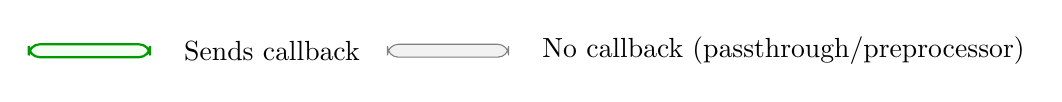
\begin{tikzpicture}[baseline]
  \node[callback, scale=0.7] (c) {};
  \node[right=0.3cm of c, anchor=west] {Sends callback};
  \node[nocallback, scale=0.7, right=3cm of c] (n) {};
  \node[right=0.3cm of n, anchor=west] {No callback (passthrough/preprocessor)};
\end{tikzpicture}

\end{document}
